
% ----------------------------------------------------------------------
%  Set the document class
% ----------------------------------------------------------------------
\documentclass[11pt,a4paper,twoside]{article}

% ----------------------------------------------------------------------
% Define external packages, language, margins, fonts and new commands
% ----------------------------------------------------------------------
%\input{preamble} 
\usepackage[utf8]{inputenc}   % <<<<< Linux
\usepackage[english]{babel} % <<<<< English
\usepackage{notoccite}
\usepackage[skip=0.5\baselineskip]{caption}
\hyphenation{GTKWave}
\usepackage{listings}
\usepackage{amsmath, bm}
\usepackage[all]{nowidow}
\usepackage[table,xcdraw]{xcolor}
\usepackage[pdf]{pstricks}

%blind text
\usepackage{graphicx}
\graphicspath{{./}{../../figlib/}{../mat/}{../sim/}}
\def\FontLn{% 16 pt normal
  \usefont{T1}{phv}{m}{n}\fontsize{16pt}{16pt}\selectfont}
\def\FontLb{% 16 pt bold
  \usefont{T1}{phv}{b}{n}\fontsize{16pt}{16pt}\selectfont}
\def\FontMn{% 14 pt normal
  \usefont{T1}{phv}{m}{n}\fontsize{14pt}{14pt}\selectfont}
\def\FontMb{% 14 pt bold
  \usefont{T1}{phv}{b}{n}\fontsize{14pt}{14pt}\selectfont}
\def\FontSn{% 12 pt normal
  \usefont{T1}{phv}{m}{n}\fontsize{12pt}{12pt}\selectfont}

% Use Arial font as default
%
\renewcommand{\rmdefault}{phv}
\renewcommand{\sfdefault}{phv}
\usepackage{geometry}	
\geometry{verbose,tmargin=2.5cm,bmargin=2.5cm,lmargin=1.15cm,rmargin=1.15cm}

%\usepackage{setspace}
%\renewcommand{\baselinestretch}{1.5}

\usepackage[pdftex]{hyperref} % enhance documents that are to be
                              % output as HTML and PDF
\hypersetup{colorlinks,       % color text of links and anchors,
                              % eliminates borders around links
%            linkcolor=red,    % color for normal internal links
            linkcolor=black,  % color for normal internal links
            anchorcolor=black,% color for anchor text
%            citecolor=green,  % color for bibliographical citations
            citecolor=black,  % color for bibliographical citations
%            filecolor=magenta,% color for URLs which open local files
            filecolor=black,  % color for URLs which open local files
%            menucolor=red,    % color for Acrobat menu items
            menucolor=black,  % color for Acrobat menu items
%            pagecolor=red,    % color for links to other pages
            pagecolor=black,  % color for links to other pages
%            urlcolor=cyan,    % color for linked URLs
            urlcolor=black,   % color for linked URLs
	          bookmarks=true,         % create PDF bookmarks
	          bookmarksopen=false,    % don't expand bookmarks
	          bookmarksnumbered=true, % number bookmarks
	          pdftitle={report},
            pdfauthor={Andre C. Marta},
%            pdfsubject={Thesis Title},
%            pdfkeywords={Thesis Keywords},
            pdfstartview=FitV,
            pdfdisplaydoctitle=true}

\usepackage[numbers,sort&compress]{natbib} % <<<<< References in numbered list [1],[2],...
\usepackage{subcaption} 
\usepackage{mdframed}

%%%%%%%%%%%%%%%%%%%%%%%%%%%%%%%%%%%%%%%%%%%%%%%%%%%%%%%%%%%%%%%%%%%%%%%%
%     Begin Document                                                   %
%%%%%%%%%%%%%%%%%%%%%%%%%%%%%%%%%%%%%%%%%%%%%%%%%%%%%%%%%%%%%%%%%%%%%%%%


\begin{document}

% Set plain page style (no headers, footer with centered page number)
\pagestyle{plain}

% Set roman numbering (i,ii,...) before the start of chapters
%\pagenumbering{roman}

% ----------------------------------------------------------------------
%  Cover page
% ----------------------------------------------------------------------
%%%%%%%%%%%%%%%%%%%%%%%%%%%%%%%%%%%%%%%%%%%%%%%%%%%%%%%%%%%%%%%%%%%%%%%%
%                                                                      %
%     File: Thesis_FrontCover.tex                                      %
%     Tex Master: Thesis.tex                                           %
%                                                                      %
%     Author: Andre C. Marta                                           %
%     Last modified :  2 Jul 2015                                      %
%                                                                      %
%%%%%%%%%%%%%%%%%%%%%%%%%%%%%%%%%%%%%%%%%%%%%%%%%%%%%%%%%%%%%%%%%%%%%%%%

\thispagestyle {empty}

% IST Logo - Signature A
% parameters: bb=llx lly urx ury (bounding box), width=h_length, height=v_length, angle=angle, scale=factor, clip=true/false, draft=true/false. 
\includegraphics[bb=9.5cm 11cm 0cm 0cm,scale=0.29]{IST_A_CMYK_POS}

\begin{center}
%
% Figure (Image or plot)
\vspace{1.0cm}
% height = 50 mm
%\includegraphics[height=50mm]{Figures/Airbus_A350.jpg}

% Title, author and degree
\vspace{1cm}
{\FontLb Circuit Theory and Electronics Fundamentals} \\ % <<<<< EDIT TITLE
\vspace{1cm}
{\FontSn Integrated Masters in Aerospace Engennering, Técnico, University of Lisbon} \\ % <<<<< EDIT COURSE
\vspace{1cm}
{\FontSn Laboratory Report 5- Bandpass Filter, Group 28} \\
\vspace{1cm}
{\FontSn Beatriz Pedroso 95773, Teresa Gonçalves 95826, Tiago Escalda 95851}\\
\vspace{1cm}
{\FontSn 6th June, 2021} \\ % <<<<< EDIT DATE (corresponds to date of oral examination)
%
\end{center}


\newpage

% ----------------------------------------------------------------------
% Dedication page (optional)
% ----------------------------------------------------------------------
%\input{dedication} 
%\cleardoublepage

% ----------------------------------------------------------------------
%  Acknowledgments (optional)
% ----------------------------------------------------------------------
%\input{acknowledgements}
%\cleardoublepage

% ----------------------------------------------------------------------
%  Abstract (both in English and Portuguese)
% ----------------------------------------------------------------------
%\input{resumo} 
%\cleardoublepage

%\input{abstract} 

% ----------------------------------------------------------------------
%  Table of contents, list of tables, list of figures and nomenclature
% ----------------------------------------------------------------------

% Table of contents
%
\tableofcontents
\newpage

% List of tables
%\addcontentsline{toc}{section}{\listtablename}
%\listoftables
%\cleardoublepage 

% List of figures
%\addcontentsline{toc}{section}{\listfigurename}
%\listoffigures
%\cleardoublepage 

% Set arabic numbering (1,2,...) after preface
%
%\setcounter{page}{1}
%\pagenumbering{arabic}

% ----------------------------------------------------------------------
%  Body
% ----------------------------------------------------------------------

\section{Introduction}
\label{introduction}


% state the learning objective
\par The aim of this laboratory assignment was to create an audio amplifier circuit. To do so, both the gain and the output stages were designed. This amplifier receives an audio maximum input of 10mV and connects to an 8 Ohm speaker. The source has an impedance of 100 Ohms and the circuit is supplied by a 12V Voltage DC source (vcc).
\par In the gain stage mentioned above, a NPN transistor and a common emitter amplifier with degeneration were used. It allows us to have a high $Z_{i}$ and a high $A_{V}$. Nevertheless, $Z_{o}$ is also very high, which consitutes a problem. Hence, this situation has to be adressed in the output stage. Consequently, in this second stage, it was used a common collecter amplifier and a PNP transistor. Not only does it allow to remain a high $A_{V}$ but it also reduces the value of $(Z_{o})$ significantly. Therefore, the gain is $\approx 1$, which is the desired result.

\par The quality of the audio amplifier is evaluated by the following expression:
\begin {equation}
	 MERIT = \frac{Voltage Gain*Bandwidth}{Cost*Lower Cut Off Frequency}   	
	\label{merit}
\end{equation}

The circuit is shown below.

\begin{figure}[ht] \centering
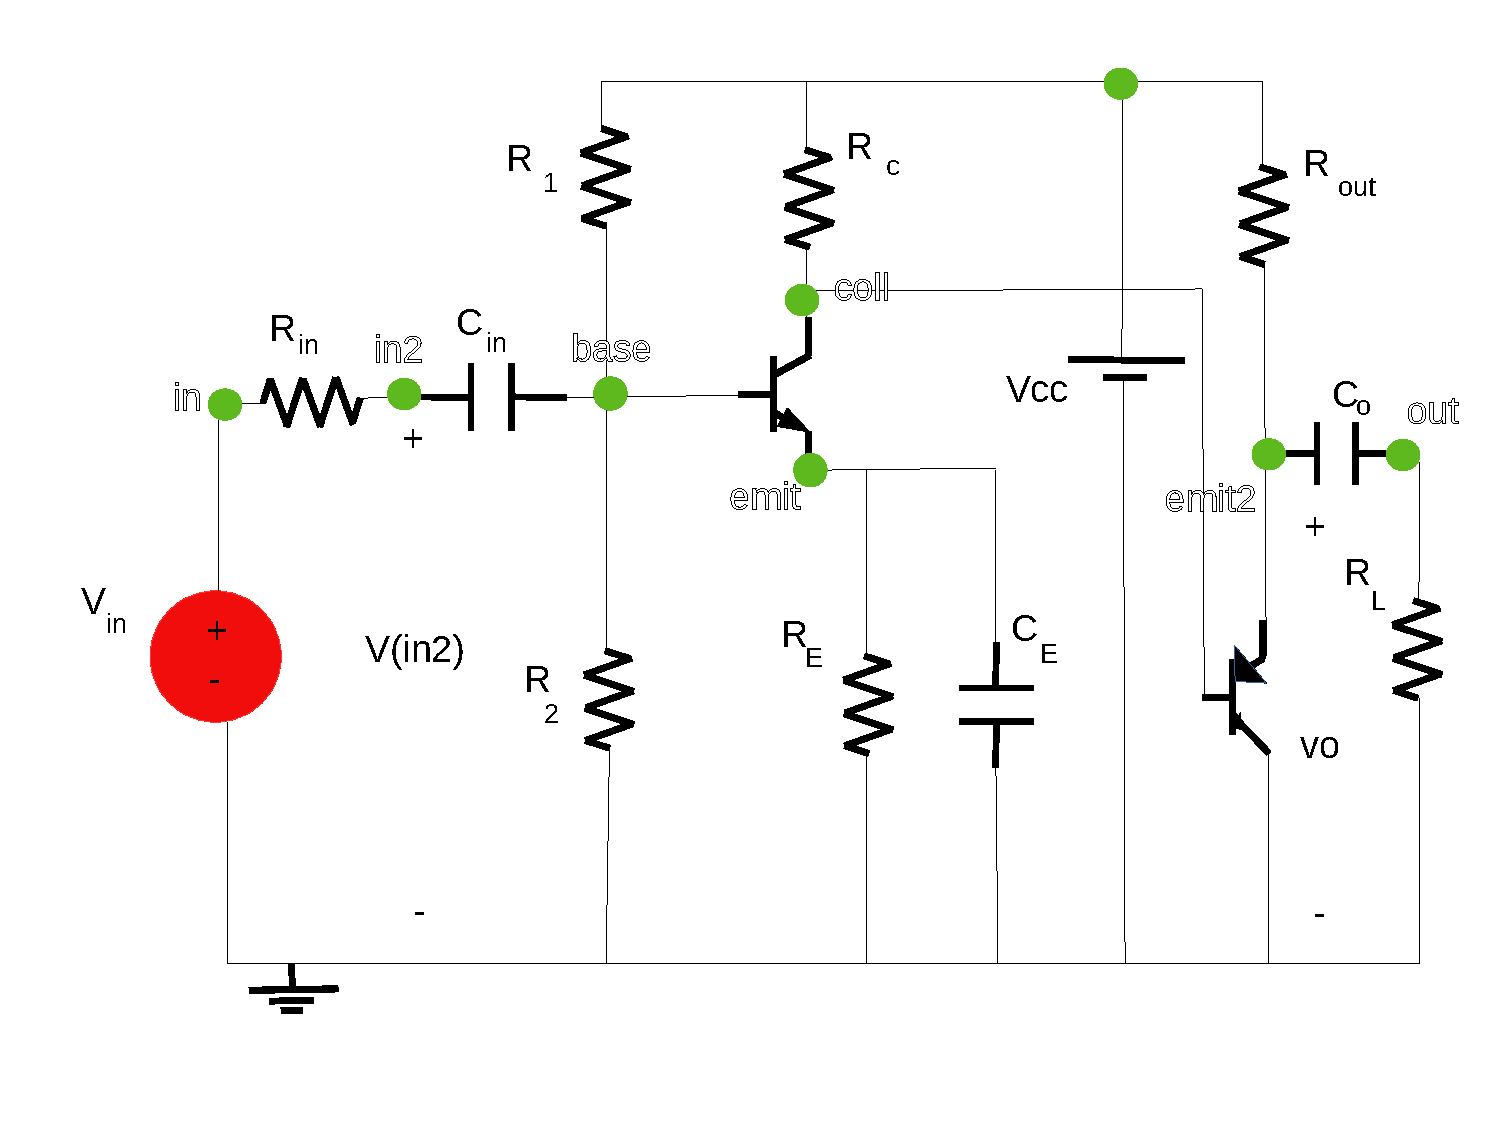
\includegraphics[width=0.8\linewidth]{lab4.pdf}
\caption{Circuit in analysis.}
\label{circuito todo}
\end{figure}


\newpage

\clearpage

\section{Theoretical Analysis} \label{section:theo}


\subsection{Node analysis for t$<$0}

\par In this section, a theoretical analysis of the circuit was conducted. The node method was the chosen approach.

The aim of using this method is to determine every node voltage. To do so, the node 4 was considered a reference node. Then, eight independent equations were written in orther to find the remaining unknown node voltage values. Before $t=0s$, v(s) is constant. Therefore, the capacitor behaves like an open-circuit which means Ix=0. The currents in the branches were also computed.


The equations were then put in the form of the matrix shown below. Octave math tools were used to solve the system.



$\begin{bmatrix}
1 & 0 & 0 & 0 & 0 & 0 & 0 & 0\\
-G1 & G1+G2+G3 & -G2 & 0 & -G3 & 0 & 0 & 0\\
0 &-Kb-G2 & G2 & 0 & Kb & 0 & 0 & 0\\
0 & 0 & 0 & 1 & 0 & 0 & 0 & 0\\
0 & -G3 & 0 & -G4 & G3+G4+G5 & -G5 & -G7 & G7\\
0 & Kb & 0 & 0 & -Kb-G5 & G5 & 0 & 0\\
0 & 0 & 0 & -G6 & 0 & 0 & G6+G7 & -G7\\
0 & 0 & 0 & Kd*G6 & -1 & 0 & -Kd*G6 & 1\\
\end{bmatrix}
$$\begin{bmatrix}
V1 \\ V2 \\ V3 \\ V4 \\ V5 \\ V6 \\ V7 \\ V8
\end{bmatrix}$
=
$\begin{bmatrix}
Vs \\ 0 \\ 0 \\ 0 \\ 0 \\ 0 \\ 0 \\ 0
\end{bmatrix}
$

\begin{table}[ht]
  \centering
  \begin{tabular}{|l|r|}
    \hline    
    {\bf Name} & {\bf Value} \\ \hline
    V1 & 5.068716e+00 \\ \hline
V2 & 4.843672e+00 \\ \hline
V3 & 4.369060e+00 \\ \hline
V4 & 0.000000e+00 \\ \hline
V5 & 4.874693e+00 \\ \hline
V6 & 5.579017e+00 \\ \hline
V7 & -1.980764e+00 \\ \hline
V8 & -2.974577e+00 \\ \hline

  \end{tabular}
  \caption{Theoretical nodal voltage results. All variables are expressed in V or A.}
  \label{tab:p2}
\end{table}


\subsection{Calculus of $R_{eq}$}
\label{subsection:2.2}

\par The purpose of this task was to compute the Req (equivalant resistance) of the circuit.

It is known that:
\begin{equation}
R_{eq}=\frac{V_{x}}{I_{x}}
\end{equation}

In order to determine the variable aforementioned, first it was sugested to calculate it seen from the capacitors terminals. Then, using the Thevenin and Norton theorem, we put the independent voltage source to 0V. $V_{x}$ is equivalent to Thevenin's Voltage, and $I_{x}$ to Norton's Current. This is necessary because the depedent voltage short cannot be put equal to 0V(short-circuit) and the independent current source cannot be erased from the circuit.
\par An ilustration of the circuit analysed is showed in figure \ref{sim2draw} 
\begin{figure}[h] \centering
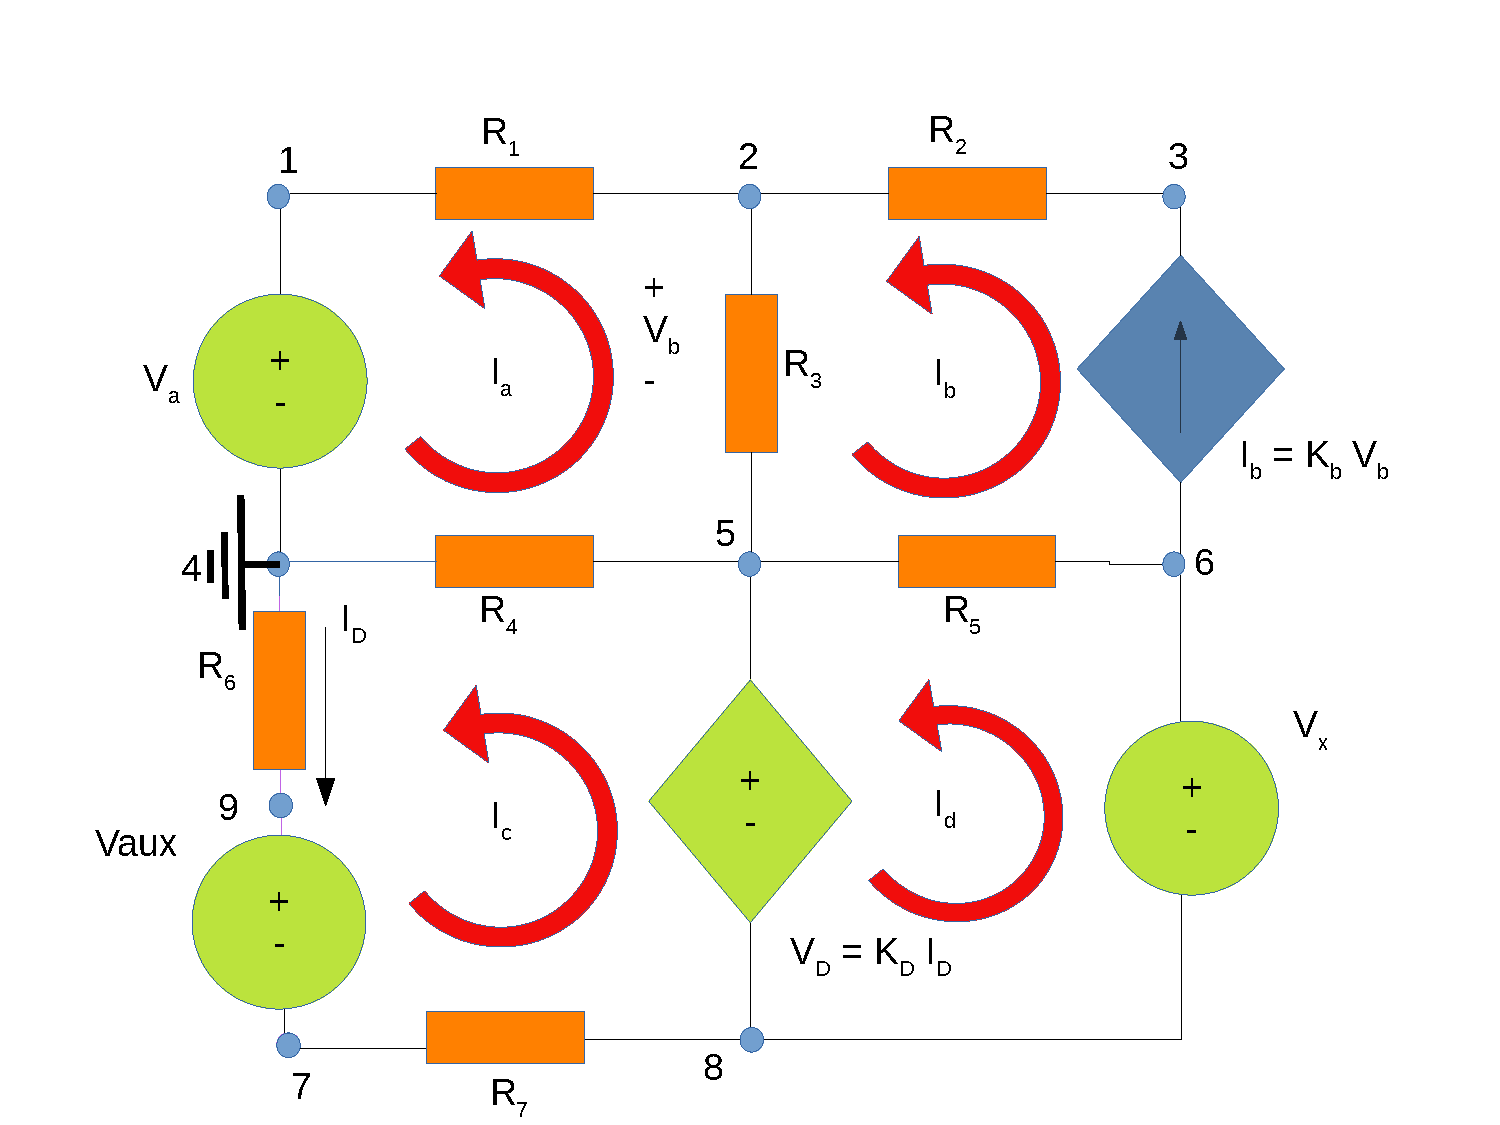
\includegraphics[width=0.65\linewidth]{sim2draw.pdf}
\caption{RC Circuit analysed in section 2.}
\label{sim2draw}
\end{figure}
\par
Then, the values of current of  every branch and the nodal values are obtained using node method. The matrix used in octave is the one that follows.

$\begin{bmatrix}
1 & 0 & 0 & 0 & 0 & 0 & 0 & 0 & 0\\
-G1 & G1+G2+G3 & -G2 & 0 & -G3 & 0 & 0 & 0 & 0\\
0 & -G2-Kb & G2 & 0 & Kb & 0 & 0 & 0 & 0\\
0 & 0 & 0 & 1 & 0 & 0 & 0 & 0 & 0\\
0 & -G1 & 0 & 0 & -G4 & 0 & -G6 & 0 & 0\\
0 & Kb & 0 & 0 & -G5-Kb & G5 & 0 & 0 & 1\\
0 & 0 & 0 & 0 & 0 & 0 & G6+G7& -G7 & 0\\
0 & 0 & 0 & 0 & 0 & 1 & 0 & -1 & 0\\
0 & 0 & 0 & KdG6 & -1 & 0 & -Kd*G6 & 1 & 0
\end{bmatrix}$
$\begin{bmatrix}
V1 \\ V2 \\ V3 \\ V4 \\ V5 \\ V6 \\ V7 \\ V8 \\ I_{x}
\end{bmatrix}$
= 
$\begin{bmatrix}
0 \\ 0 \\ 0 \\ 0 \\ 0 \\ 0 \\ 0 \\ V_{x} \\ 0
\end{bmatrix}$

\par Theoretically speaking, once the voltage source is equal to 0V, $V_{4}$ and  $V_{1}$ are also to be 0. 

\begin{table}[]
  \centering
  \begin{tabular}{|l|r|}
    \hline    
    {\bf Name} & {\bf Value} \\ \hline
    V1 & 0.000000e+00 \\ \hline
V2 & 0.000000e+00 \\ \hline
V3 & 9.496396e-16 \\ \hline
V4 & 0.000000e+00 \\ \hline
V5 & 5.935248e-17 \\ \hline
V6 & 8.553593e+00 \\ \hline
V7 & -2.967624e-17 \\ \hline
V8 & 0.000000e+00 \\ \hline
Ix & -2.745419e-03 \\ \hline
Req & 3.115588e+03 \\ \hline
tau & 3.244185e-03 \\ \hline

  \end{tabular}
  \caption{Theoretical nodal voltage results. All variables are expressed in Volt, Ampere or Ohm.}
  \label{tab:p2}
\end{table}


\clearpage

\subsection{Node analysis for t $\ge$ 0 (Natural solution)}


It was proposed to study and determine the natural response of the circuit over time, in node 6. The natural response is what the circuit does including the initial conditions (initial voltage of the capacitor) but with the imput supressed. 

In order to calculate the natural solution, we have to eliminate the voltage source, which means vs(t)=0V. Hence, we have an equivalent cicuit described by a voltage source and the capacitor. The voltage V8=0V and the amplitude $Vx=V6-V8=V6$. Over the time, the voltage $V{6n}$ is decreasing which means the capacitor is discharging. The natural solution will have the format $V{6n}(t)=A*e^{(-t/tau)}$ with $tau=Req*C$ and $A=V6$ obtained in \ref{subsection:2.2}. As expected, the result is a negative exponencial graph, shown bellow.

\begin{figure}[ht] \centering
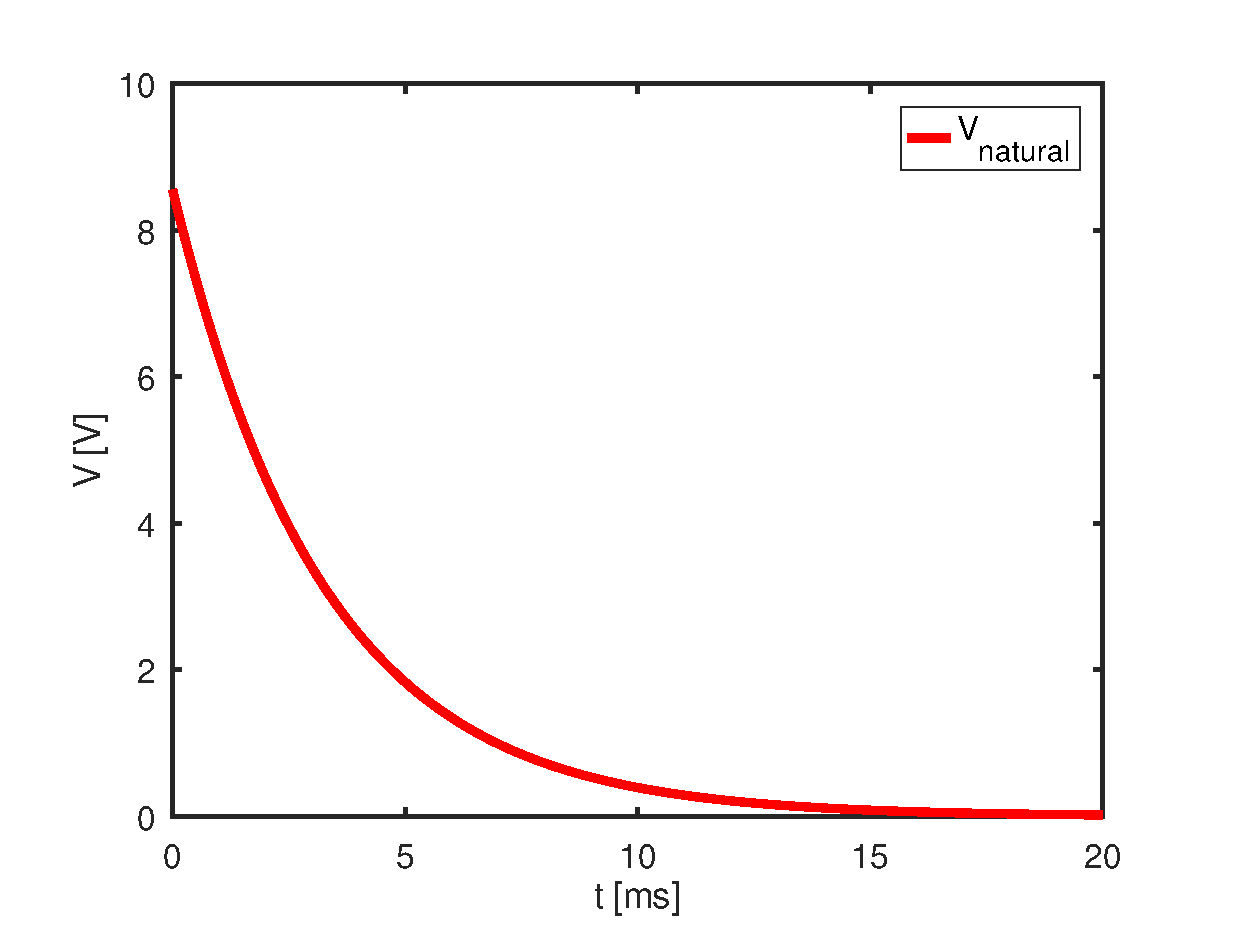
\includegraphics[width=0.5\linewidth]{natural.eps}
\caption{Circuit analysed.}
\label{fig:sim3}
\end{figure}



\subsection{Node analysis for t $\ge$ 0 (Forced solution)}

The forced response of a circuit is calculated with the sources turned on, but with the initial conditions (internal stored energy) set to zero.What is forced response? The forced response is where the output (the voltage on the capacitor) is going to end up in the long run after all stored energy eventually dissipates. The forced response does this by ignoring the presence of energy storage elements (in this case, it ignores the capacitor and its initial voltage). However, the forced response can't tell us what happens at t=0, or during the transition to the final state, because it ignores the stored energy. 
\par Like so, a phasor was used, with $V_{s}=1$. The capacitor was replaced by its impiedence $Z$. Then, the nodal method was run again, with this new variable.
\begin{equation}
w=2*pi*f
\end{equation} 

\begin{equation}
Zc=1/(j*w*C);
\end{equation} 

\par The matrix used was the following:

$\begin{bmatrix}
1 & 0 & 0 & -1 & 0 & 0 & 0 & 0 \\
-G1 & G1+G2+G3 & -G2 & 0 & -G3 & 0 & 0 & 0 \\
0 & -G2-Kb & G2 & 0 & Kb & 0 & 0 & 0 \\
0 & 0 & 0 & 1 & 0 & 0 & 0 & 0 \\
0 & G3 & 0 & G4 &-G3-G5-G4 & G5+1/Zc & G7 & -G7-1/Z_{c}\\
0 & Kb & 0 & 0 & -G5-Kb & G5+1/Z_{c} & 0 & -1/Z_{c} \\
0 & 0 & 0 & 0 & 0 & 0 & G6+G7& -G7 \\
0 & 0 & 0 & KdG6 & -1 & 0 & -Kd*G6 & 1
\end{bmatrix}$
$\begin{bmatrix}
V1 \\ V2 \\ V3 \\ V4 \\ V5 \\ V6 \\ V7 \\ V8
\end{bmatrix}$
= 
$\begin{bmatrix}
1 \\ 0 \\ 0 \\ 0 \\ 0 \\ 0 \\ 0 \\ 0 \\ 
\end{bmatrix}$
\par Then, the complex amplitudes with the knowlegde that the amplitude of the forced response is the absolute value of the complex $V_{6}$, and the phase is the argument, the forced solution is then given by:

\begin{equation}
V6_f=A*sin(w*t+Ph)
\end{equation} 

\par The tables below present the values that allows us to compute the comlex amplitude of every node voltage. In fact, it is obtained by the following expression: 

\begin{equation}
V_{complex}(i)=V_i exp(-j*phase(i))
\end{equation} 


\begin{table}[ht]

  \centering
  \begin{tabular}{|l|r|}
    \hline    
    {\bf Name} & {\bf Value [V]} \\ \hline
    V1 & 1.000000e+00 \\ \hline
V2 & 9.556014e-01 \\ \hline
V3 & 8.619659e-01 \\ \hline
V4 & 2.801649e-17 \\ \hline
V5 & 9.617215e-01 \\ \hline
V6 & 5.886212e-01 \\ \hline
V7 & 3.907822e-01 \\ \hline
V8 & 5.868501e-01 \\ \hline

  \end{tabular}
  \caption{Amplitudes of Nodal Voltages} 
\end{table}


\begin{table}[ht]

  \centering
  \begin{tabular}{|l|r|}
    \hline    
    {\bf Name} & {\bf Value [Rad]} \\ \hline
    Phase1 & 0.000000e+00 \\ \hline
Phase2 & -5.722643e-16 \\ \hline
Phase3 & -1.142921e-15 \\ \hline
Phase4 & 3.141593e+00 \\ \hline
Phase5 & -5.388346e-16 \\ \hline
Phase6 & -3.000819e+00 \\ \hline
Phase7 & 3.141593e+00 \\ \hline
Phase8 & 3.141593e+00 \\ \hline

  \end{tabular}
  \caption{Phase of Nodal Voltages} 
\end{table}




\newpage



\subsection{Natural and Forced Superimposed}


The total response of a circuit can be teased apart into a forced response plus a natural response. These responses can be combined using the principle of superposition. This principle pressupose the addition of the natural response and the forced response, both calculated in question 3 and 4.

The final solution for $V(6)_{final}$  is then given by:


\begin{equation}
V6_{final}
\begin{cases}
V_{6}-V_{8} & $t$ < $0$ \\
V(6)_{n} + A*sin(w*t+Ph) & $t $\geq$ 0$
\end{cases}
\label {eq:n2}
\end{equation}



The final solution for $V(S)_{final}$  is then given by:

\begin{equation}
VS_{final}
\begin{cases}
Vs & $t$ < $0$ \\
e.^{(-j*(w*t_pos-pi/2))}& $t $\geq$ 0$
\end{cases}
\label {eq:n2}
\end{equation}


\begin{figure}[h] \centering
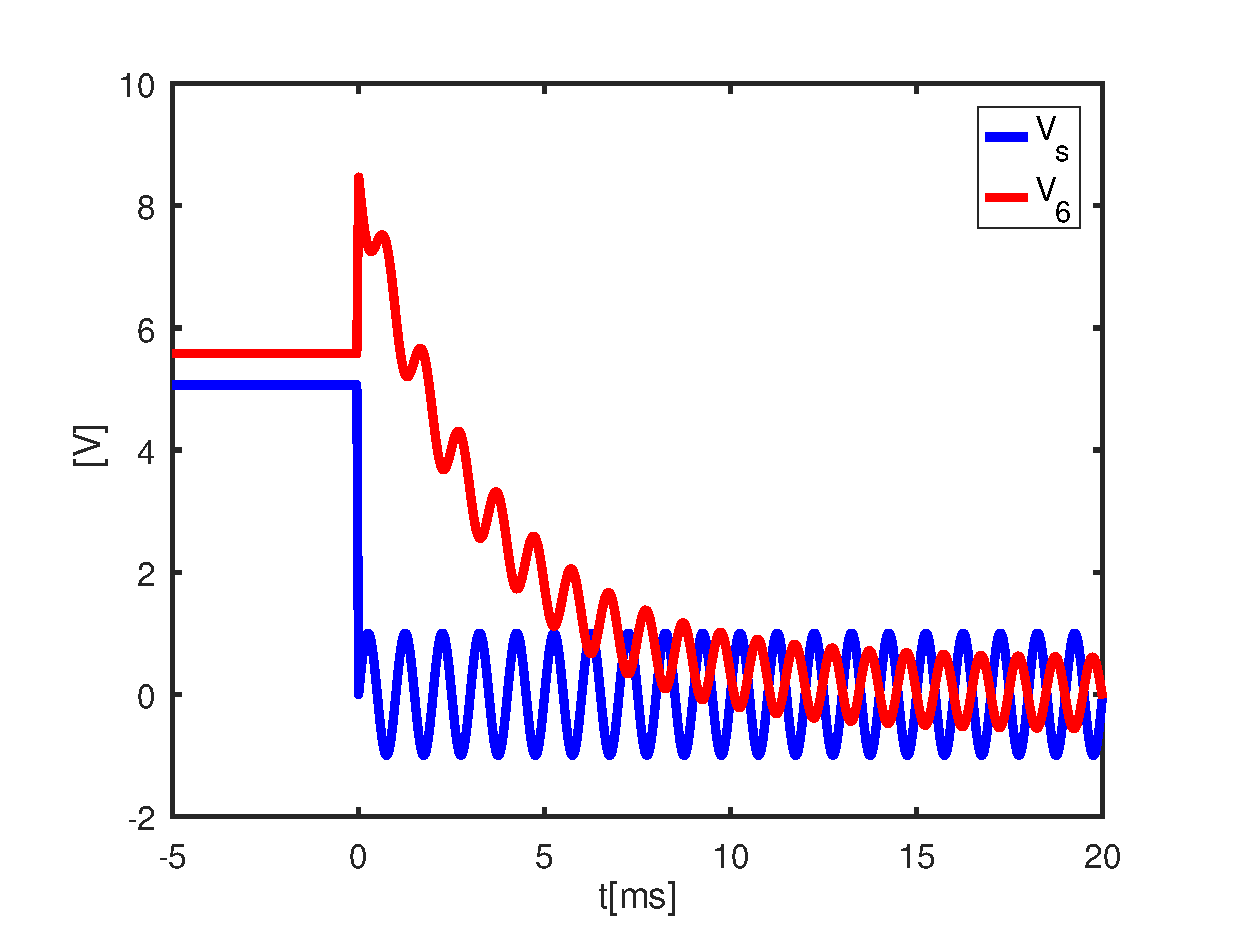
\includegraphics[width=0.6\linewidth]{part4.eps}
\caption{Final response.}
\label{fig:part4}
\end{figure}

\par It is observed in \ref{fig:part4} that $V(6)_{final}$ tends to diminuish  until 20ms, the end of the period. By this time, the phase $V(6)_{final}$ and the phase of  $VS_{final}$ differ $\pi$ or 180 degrees.




\subsection{Frequency Responses}

In this section, both octave and ngspice were used in order to obtain plots of the phase response and of the magnitude response, using logscale. This approach is very useful hence it provides a much better plot fit and, therefore it provides great visualization for users. The magnitude in debicels is of interest for analysis of sound waves, and the analysis of the phase or angle delay is a very interesting way of study another parameter to compare signal. Frequency range in both analysis was from 0.1 Hz to 1MHz. The plots made were v6(f), vs(f) and vc=(v6(f)-v8(f)).



To examine the frequency responses, the system of equations in Section 4 is solved in a loop cycle, what allows us to calculate the $V_6$, $V_c$ and $V_s$ for each frequence. For each result of these complex vectors, the values were saved.

\subsubsection{Frequency Response- Magnitude}

To represent the magnitude in dB, the absolute values were converted ($X_{dB}$=20$log_{10}$(X)). The frequencies were put in a logarithmic scale.

The magnitude of $V_s$ does not suffer any alteration with the variation of the frequency of the signal. Since its amplitude is 1, as one can observe in the graphics shown at the end of the section, the plot shows a constant horizontal line, with the value zero (0=$log_{10}$(1)).

On the contrary, as the frequency is increasing, the magnitudes of $V_6$ and $V_c$ decrease. The value of $V_c$ changes as it is expected in a RC circuit. This is due to the impedance of the capacitor (Z=-j/wC).

\begin{figure}[h] \centering
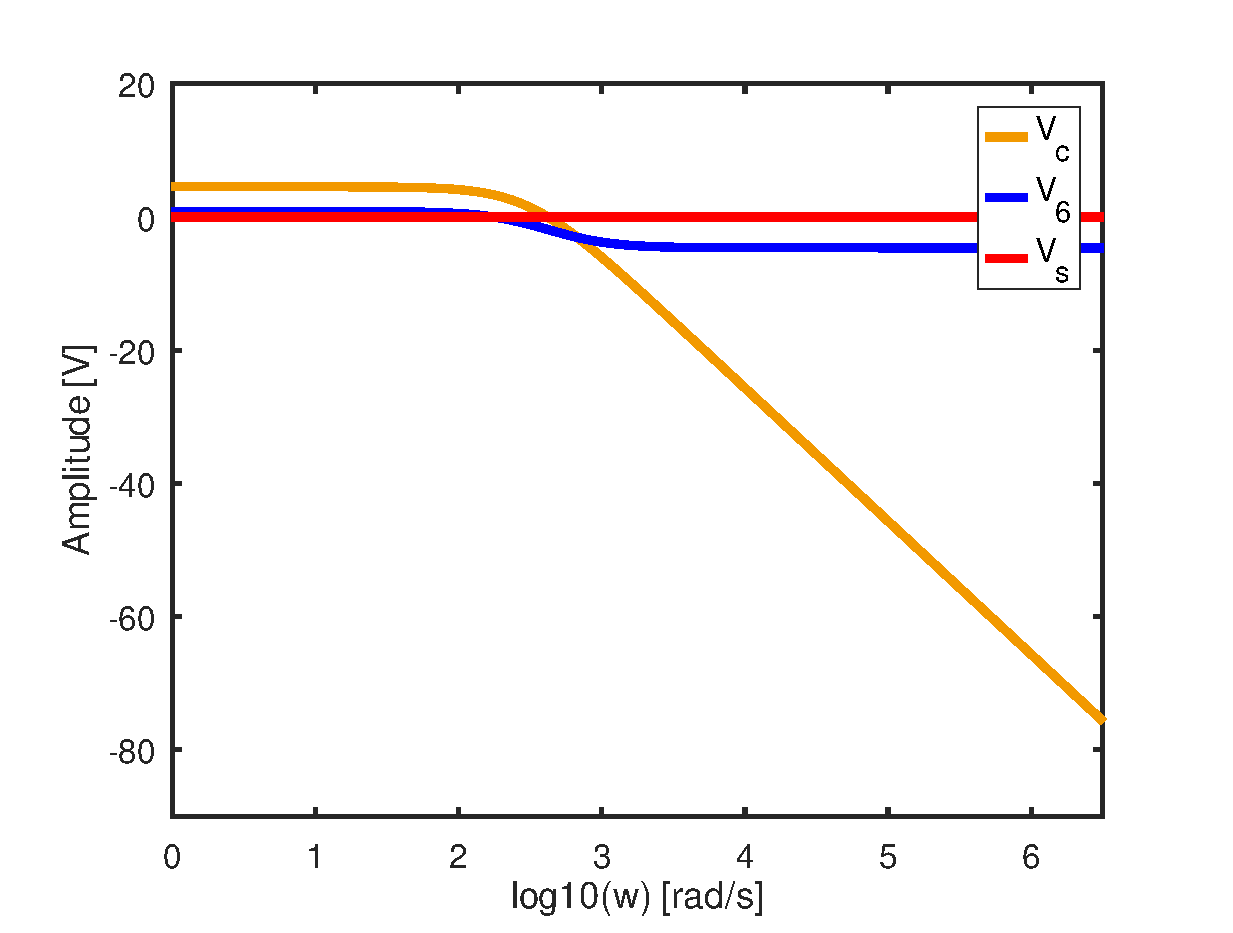
\includegraphics[width=0.5\linewidth]{part6_amp.eps}
\caption{Circuit analysed.}
\label{Magnitude response.}
\end{figure}

\subsubsection{Frequency Response- Phase}


The angles of the values saved were transformed from radians to degrees. The phase in $V_s$ is 0, therefore we do not have to do any further calculations. The phase of each voltage corresponds to the exact angles. In the plot shown below, the frequencies were also  put in the logarithmic scale. As the frequency increases the phase tend to negative values, which varies as it is expected.

\begin{figure}[ht] \centering
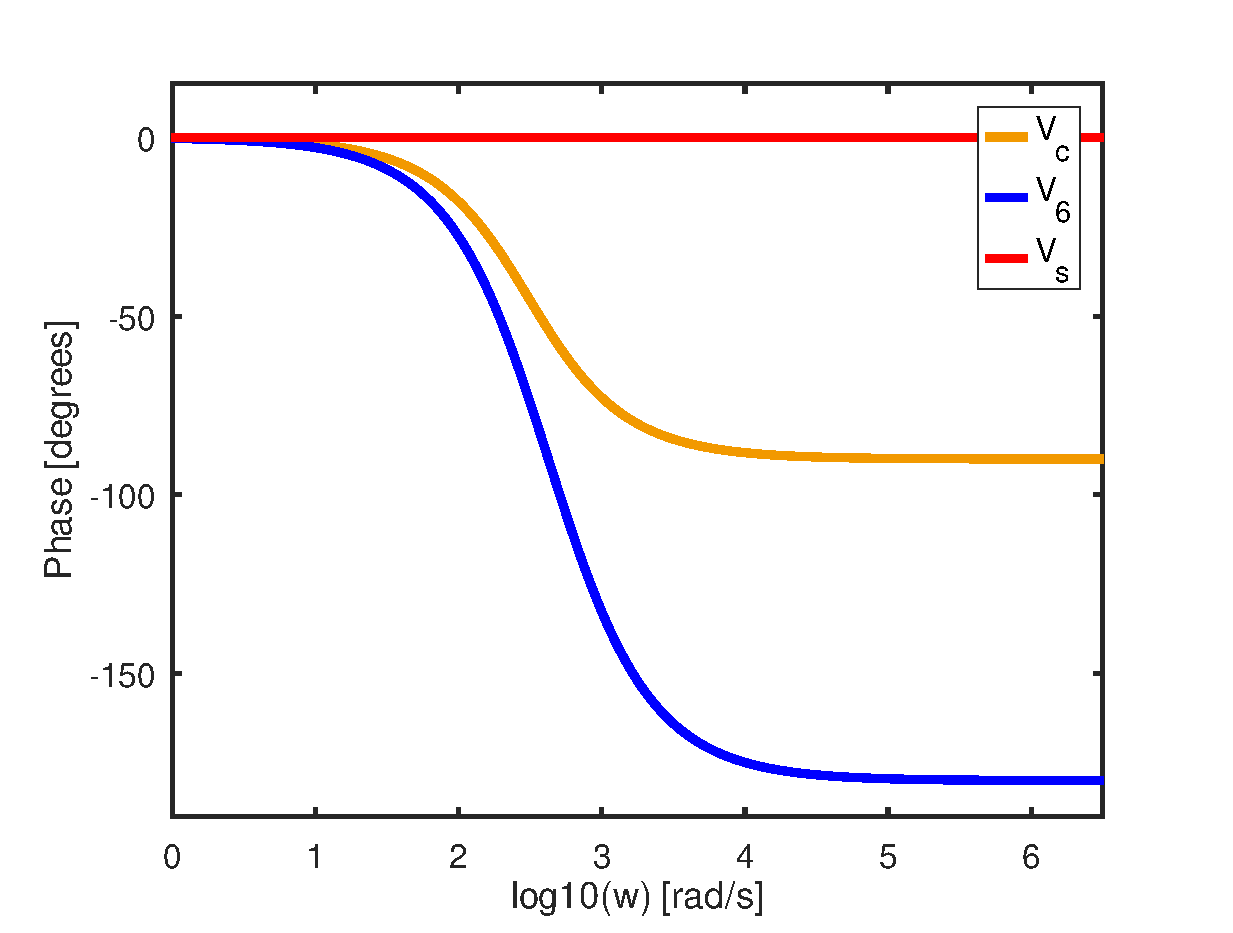
\includegraphics[width=0.5\linewidth]{part6_ang.eps}
\caption{Phase response.}
\label{RC Circuit.}
\end{figure}














\clearpage

\section{Simulation Analysis}
\label{section:sim}
 
In this section, the several steps taken using ngspice in order to conduct the simulation of the band pass filter using an OP-AMP, as requested, will be described. The main focus of the simulation was to determine and optimize the values of the gain, the central frequency and the output and input impedances. The quality and overall figure of merit will then be analysed.
The group proceded as follows:

\begin{enumerate}
\item Design of the circuit, having as a starting point the circuit presented in section \ref{introduction}

  
\item  In the frequency domain, measure of the output voltage gain, using the function .meas as well as the lower and upper cut off frequencies and the central frequency.


\begin{table}[ht]
  \centering
  \begin{tabular}{|l|r|}
    \hline    
   Gain& 34.0105\\ \hline
Central Frequency& 794.328\\ \hline
Gain deviation&49.8206\\ \hline
Central frequency deviation&205.672\\ \hline

    \end{tabular}
  \caption{Results for ngspice}
    \label{tab:results}
\end{table}


Then, the response of the circuit in dB and the phase were computed. The gain was also determined. In fact, the main goal of the assignement was to design a band pass filter. This means that this filter should cut both low an very high frequencies. THis is precisely what is shown in figure \ref{fig:gain}




\begin{figure}[ht]
\centering
\begin{subfigure}{.5\textwidth}
  \centering
  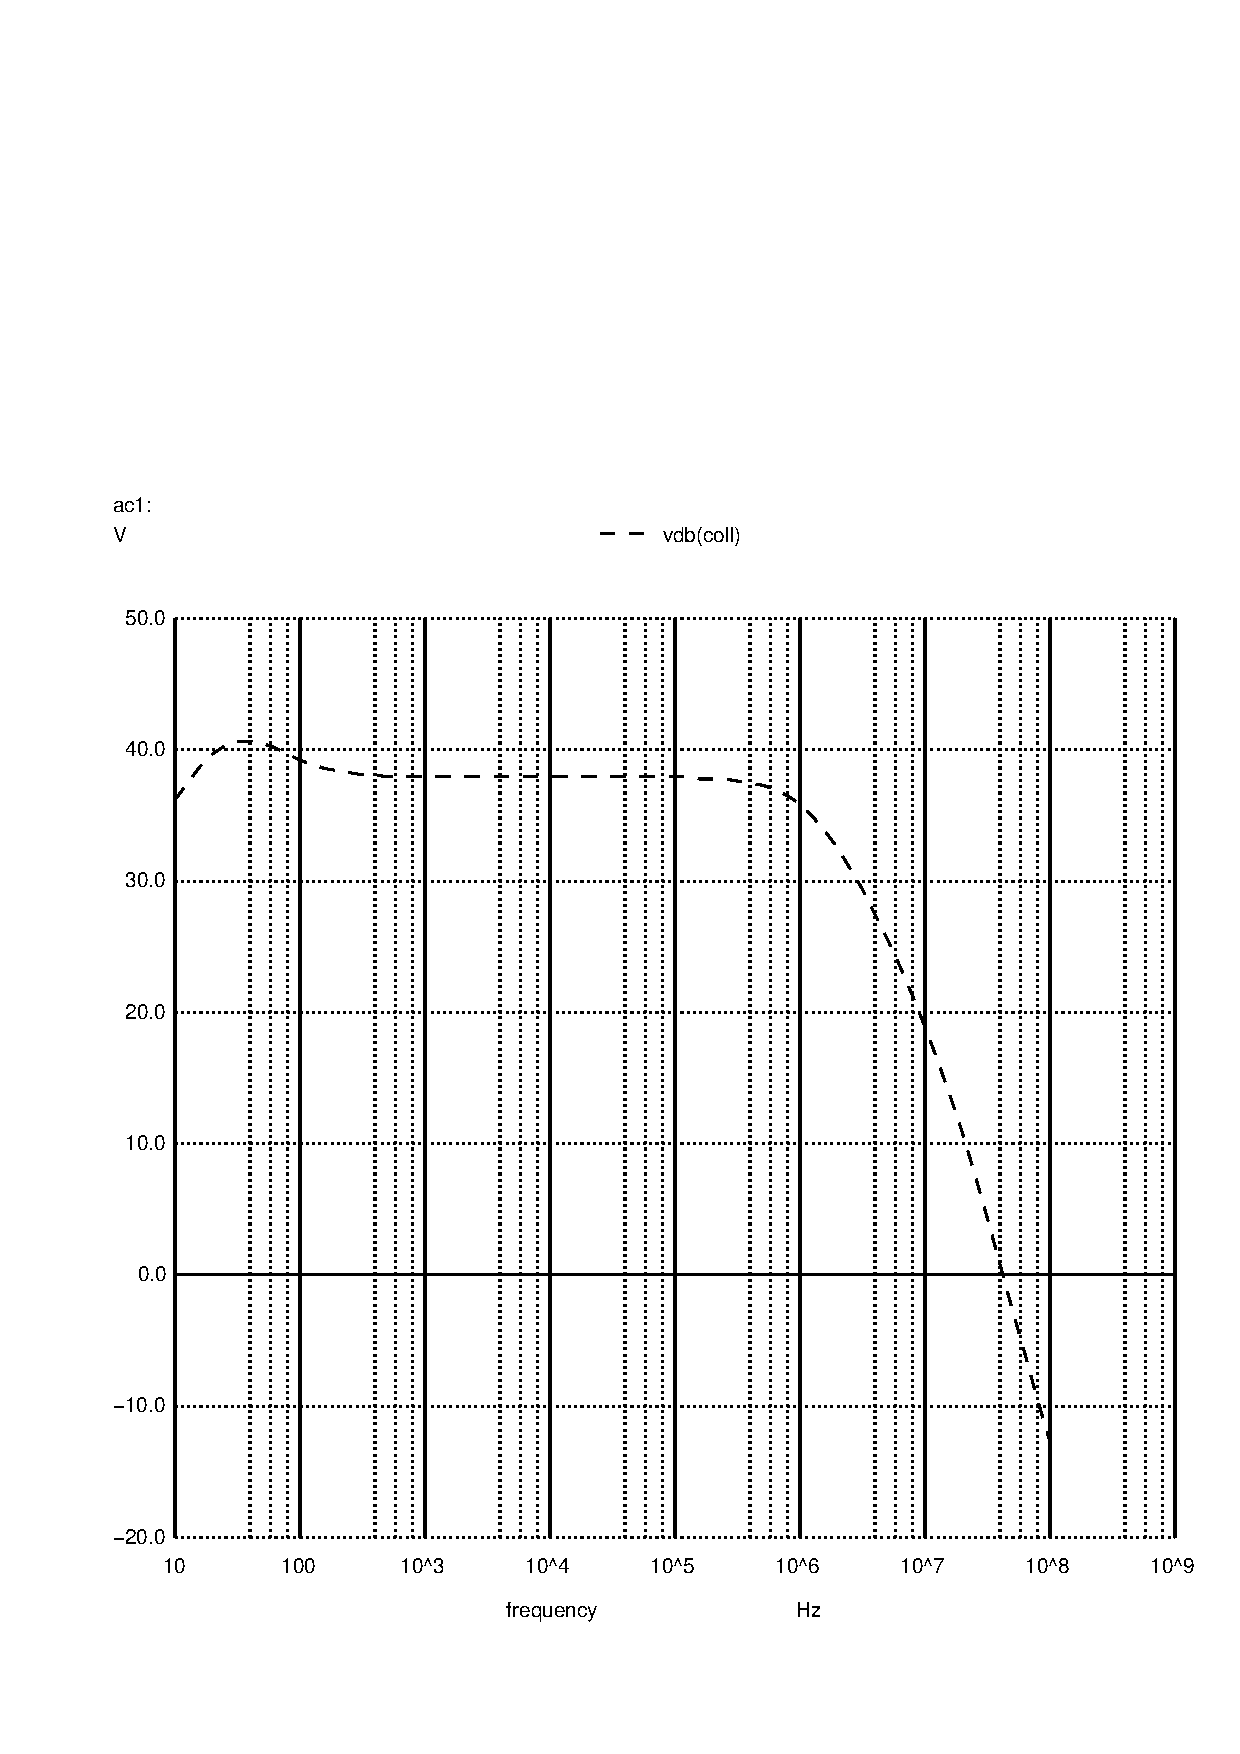
\includegraphics[width=.45\linewidth]{vo1f.pdf}
  \caption{Output Voltage in dB}
  \label{fig:sim5}
\end{subfigure}%
\begin{subfigure}{.5\textwidth}
  \centering
  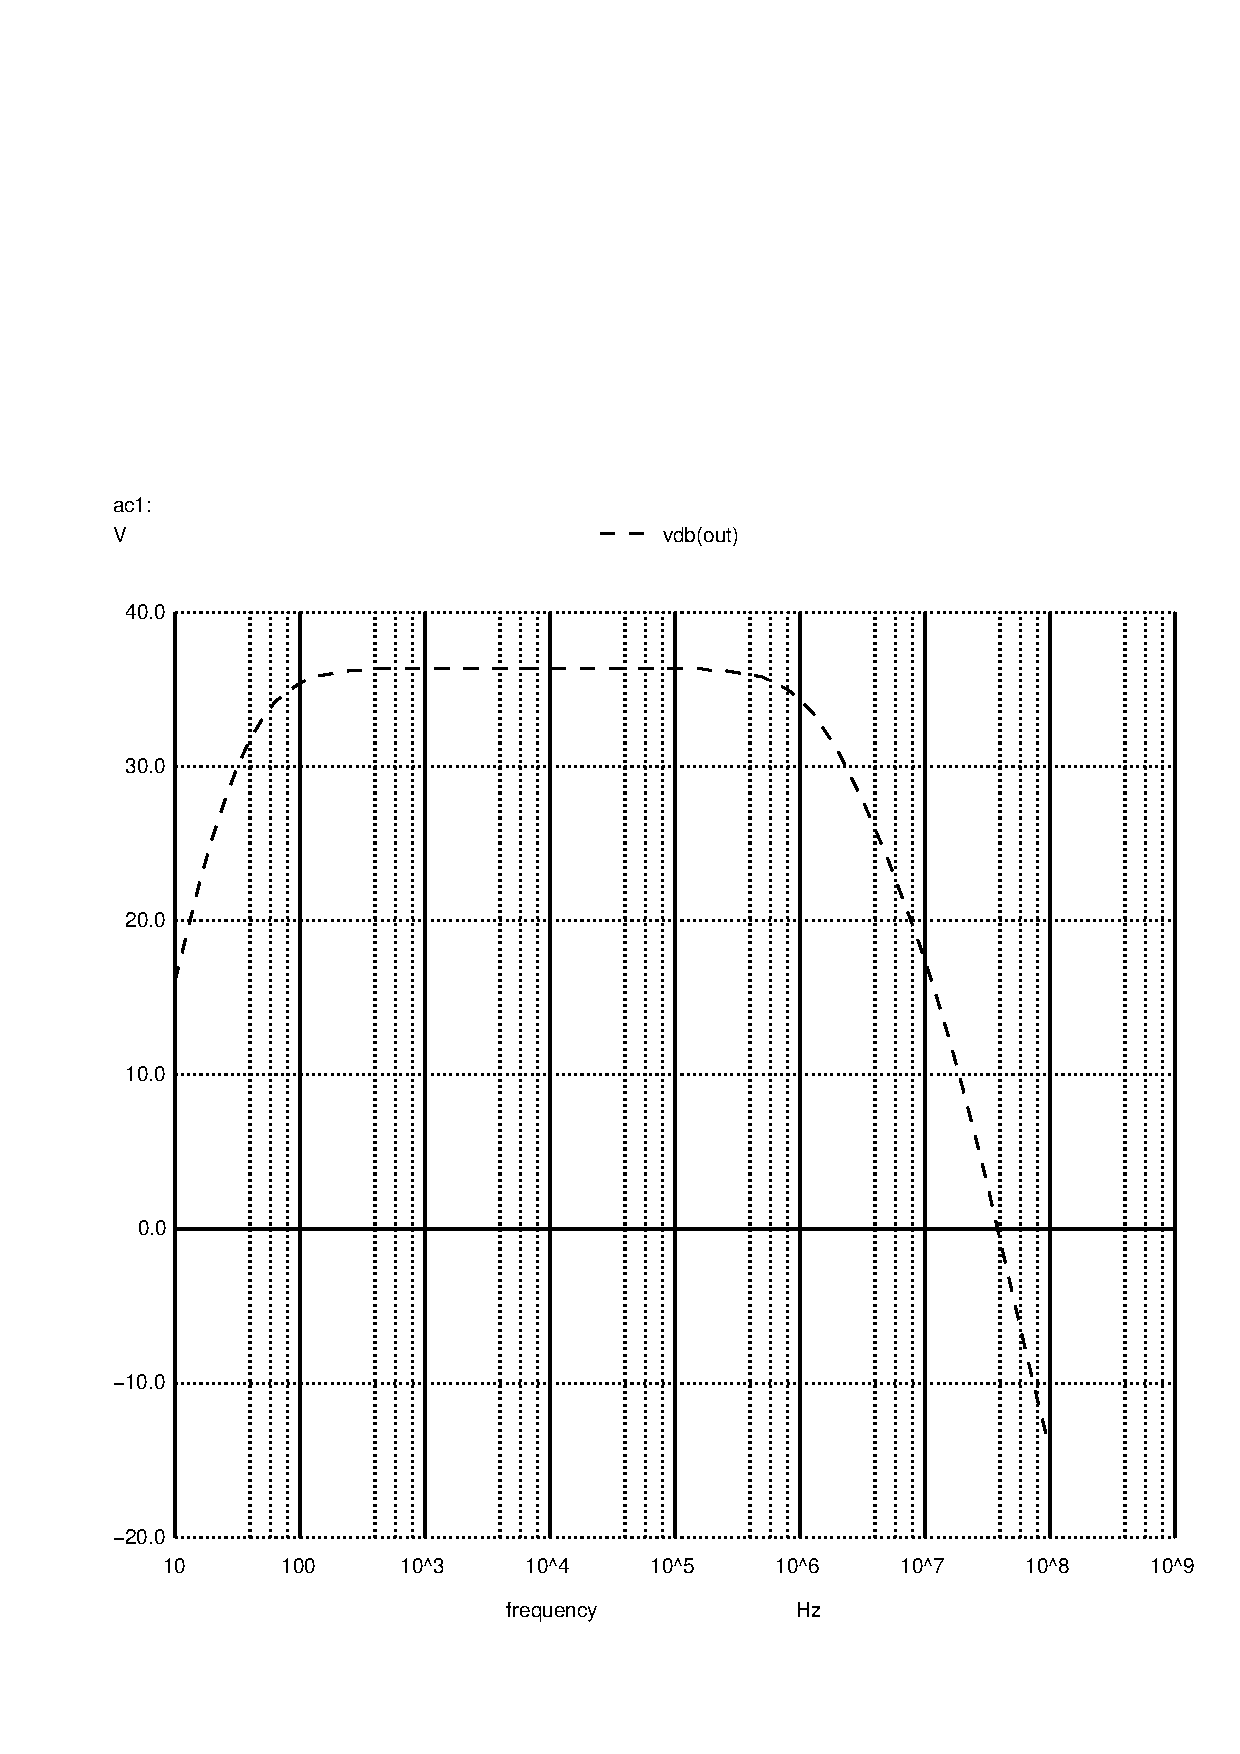
\includegraphics[width=.45\linewidth]{vo2f.pdf}
  \caption{Output voltage (phase)}
  \label{fig:sim6}
  \end{subfigure}
  \begin{subfigure}{.5\textwidth}
  \centering
  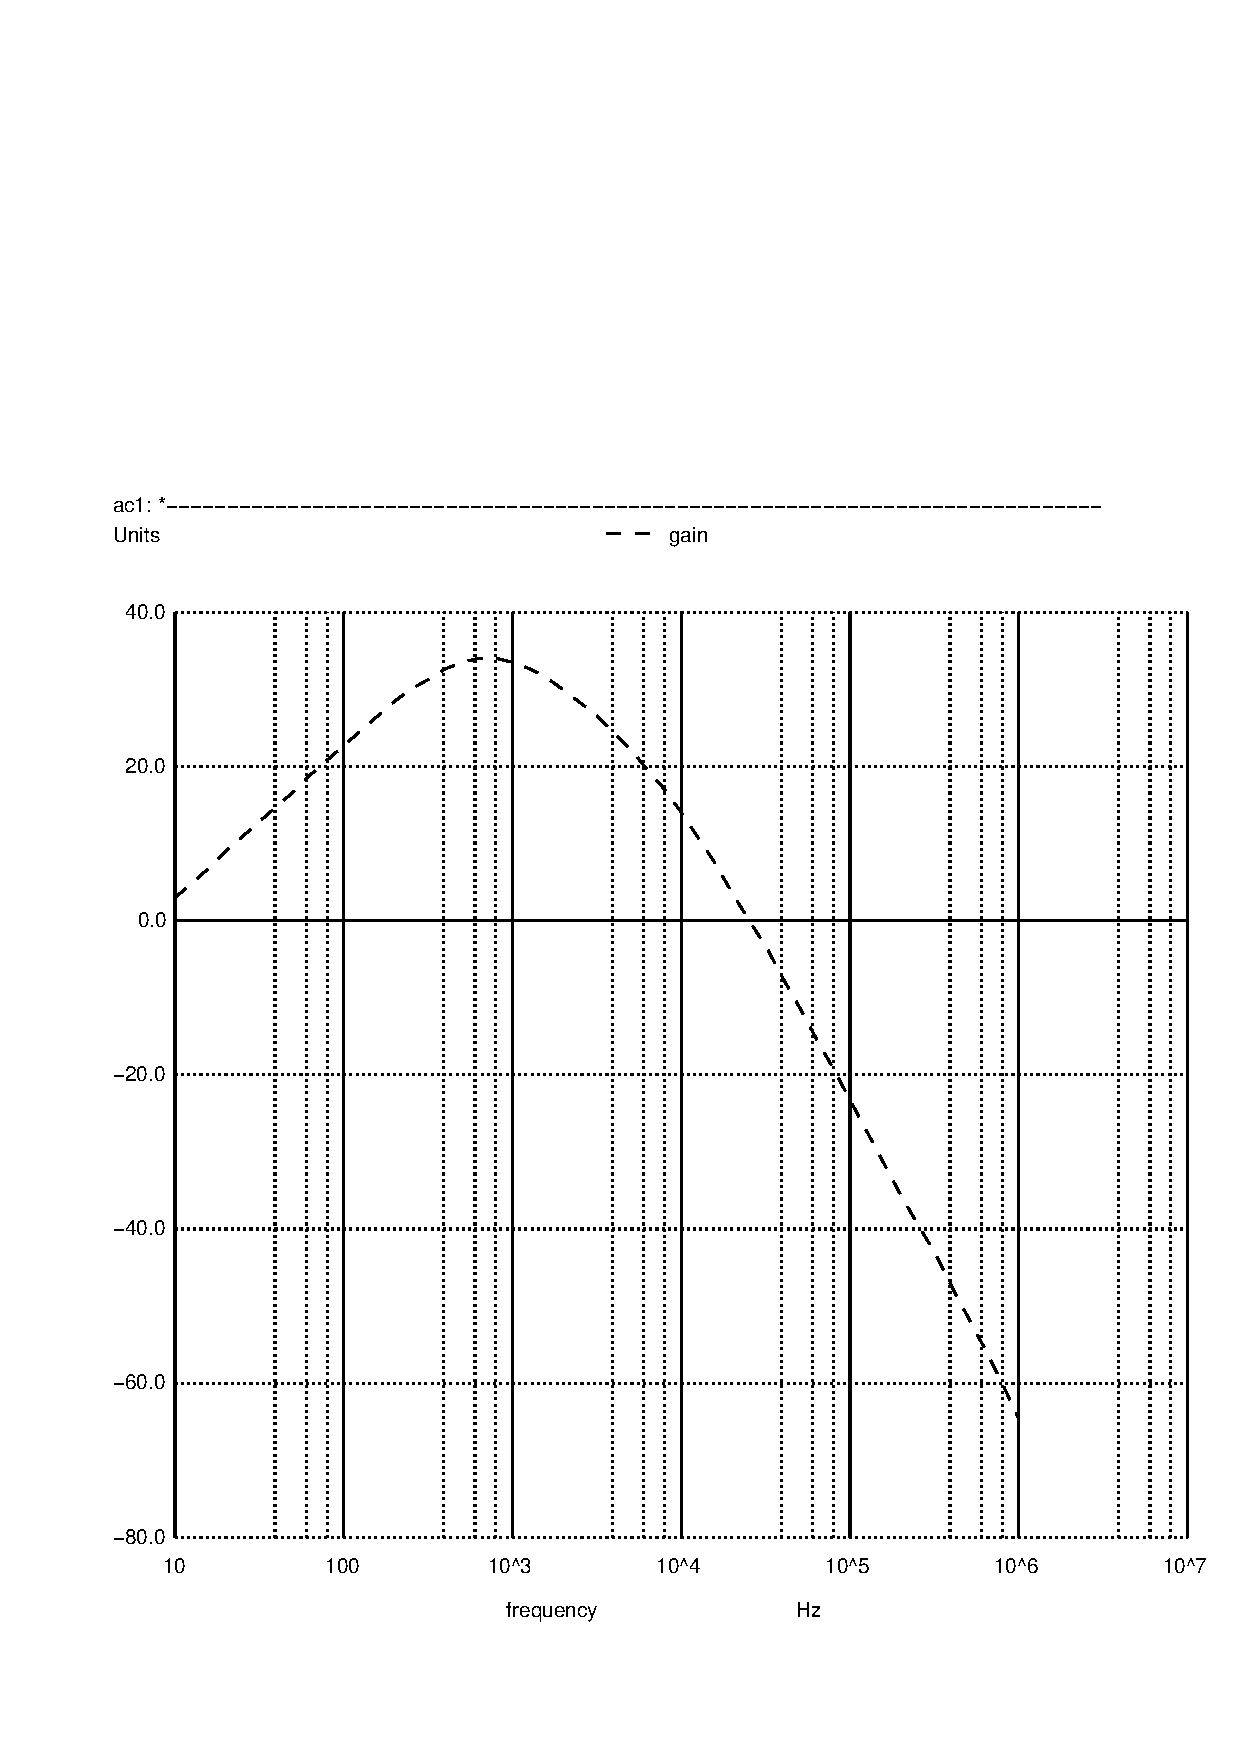
\includegraphics[width=.45\linewidth]{gain.pdf}
  \caption{Gain}
  \label{fig:sim6}

\end{subfigure}
\end{figure}



\item Determination of the input impedance, seen from the input voltage source.

\begin{table}[h]
  \centering
  \begin{tabular}{|l|r|}
    \hline    
   Zin & 999.002 + -7.3282 j\\ \hline

   \end{tabular}
  \caption{Input impedance in Ohm}
    \label{tab:ZI}
\end{table}

\par The result obtained for the input impedance, considering the value in Ohm, is high. This is benefitial for the gain, because the voltage in the node In 2 must be as similiar to Vin as possible. Using a voltage divider, the only way to achieve this was to have a very high resistance value.

\item Determination of the output impedance, using a different set up, seen from the load resistance. 

\begin{table}[h]
  \centering
  \begin{tabular}{|l|r|}
    \hline    
   Zo & 0.0522978 + -7.23396 j\\ \hline

   \end{tabular}
  \caption{Output impedance in Ohm}
  
  \label{tab:ZO}
\end{table}


Conserning the output impedance, an opposite deduction to the one made for the output impedance is mandoratory. Considering a voltage divider, the output impedance must be as low as possible, in order to the output voltage to be as high as possible. Having said that, an analysing tables \ref{tab:ZI} \ref{tab:ZO}, the difference needed between the two is confirmed. 

\item Compute of the cost and figure of merit
\par To finally understand the efficency of the amplifier, the cost and figure of merit were calculated

\begin{table}[ht]
  \centering
  \begin{tabular}{|l|r|}
    \hline    
   Cost & 1225.6\\ \hline
merit & 716.238\\ \hline

   \end{tabular}
  \caption{Cost and Figure of merit}
  \label{tab:cost}
\end{table}

Analysing table \ref{tab:cost}, the results obtained may be considered satisfying.


\end{enumerate}




\clearpage

\section{Comparison}
\label{section:comparison}

\par In this section, a comparison between Octave and Ngspice results will be made. Firstly, the operating point was computed using the theoretical DC model. In the tables below, the three current values ($I_{A}$, $I_{B}$, $I_{C}$) are presented as well as the voltage in the coll.

\begin{table}[ht]
\parbox{.45\linewidth}{
  \centering
  \begin{tabular}{|l|r|}
    \hline    
    {\bf Calculus} & {\bf Value [A or V]} \\ \hline
    @c1[i] & 0.000000e+00\\ \hline
@gb[i] & -2.26065e-04\\ \hline
@r1[i] & 2.161572e-04\\ \hline
@r2[i] & -2.26065e-04\\ \hline
@r3[i] & -9.90741e-06\\ \hline
@r4[i] & 1.183330e-03\\ \hline
@r5[i] & -2.26065e-04\\ \hline
@r6[i] & -9.67173e-04\\ \hline
@r7[i] & 9.671730e-04\\ \hline
v(1) & 5.068716e+00\\ \hline
v(2) & 4.843672e+00\\ \hline
v(3) & 4.369060e+00\\ \hline
v(5) & 4.874693e+00\\ \hline
v(6) & 5.579017e+00\\ \hline
v(7) & -1.98076e+00\\ \hline
v(8) & -2.97458e+00\\ \hline
v(9) & -1.98076e+00\\ \hline

  \end{tabular}
  \caption{Operating point using DC model. Variables are expressed in Ampere or Volt. (Ngspice)}} 
\parbox{.45\linewidth}{
 \centering
  \begin{tabular}{|l|r|}
    \hline    
    {\bf Name} & {\bf Value [A or V]} \\ \hline
    \input{../mat/ponto1_TAB}
  \end{tabular}
  \caption{Operating point using DC model. Variables are expressed in Ampere or Volt.(Octave)}}
\end{table}

As one may observe, some discrepancies are noticeable. These may be due to....


SEI LAAAAAAA FALTA ISTOOOOOOOOOOOOOOOOOOOOOOOOOOO

Moreover, the importance of this calculations must be highlighted. In fact, the theoretical gain expression is dependent on the value of the current $I_{C}$. This relation can be understood by the expression below. Since this incremental parameter is also present in the gain expression, this may be one of the reasons why some discrepancies may be observed when comparing Octave and Ngspice gain resuts. 

\begin {equation}
	 MERIT = \frac{$I_{C}$}{$V_{T}$}   	
	\label{gm_eq}
\end{equation}

\par For both stages, input and output impedances were also computed and the results are shown in the following table.

\begin{table}[ht]
\parbox{.45\linewidth}{
  \centering
  \begin{tabular}{|l|r|}
    \hline    
    {\bf Calculus} & {\bf Value [V]} \\ \hline
    \input{../sim/Zin_TAB}
  \end{tabular}
  \caption{Results for the voltage regulator. All variables are expressed in Volt. (Ngspice)}} 
\parbox{.45\linewidth}{
  \centering
  \begin{tabular}{|l|r|}
    \hline    
    {\bf Calculus} & {\bf Value [V]} \\ \hline
    \input{../sim/op_ZO_TAB}
  \end{tabular}
  \caption{Results for the voltage regulator. All variables are expressed in Volt. (Ngspice)}} 
\parbox{.45\linewidth}{
  \centering
  \begin{tabular}{|l|r|}
    \hline    
    {\bf Name} & {\bf Value [A or V]} \\ \hline
    \input{../mat/Z_TAB}
  \end{tabular}
  \caption{Results for the voltage regulator. All variables are expressed in Volt.(Octave)}}
\end{table}
 
 EXPLICAR DIFERENCAS DAS IMPEDANCIASSSSSSSSSSSSSSSSSSSSSSSSSSSSS
 
 Aditionally, the gain, bandwidth and cut off frequency results were also computed and compared.
 
 \begin{table}[ht]
\parbox{.45\linewidth}{
  \centering
  \begin{tabular}{|l|r|}
    \hline    
    {\bf Calculus} & {\bf Value} \\ \hline
    Gain& 34.0105\\ \hline
Central Frequency& 794.328\\ \hline
Gain deviation&49.8206\\ \hline
Central frequency deviation&205.672\\ \hline

  \end{tabular}
  \caption{Gain, bandwidth and cut off frequency. (Ngspice)}} 
\parbox{.45\linewidth}{
 \centering
  \begin{tabular}{|l|r|}
    \hline    
    {\bf Name} & {\bf Value} \\ \hline
    \input{../mat/r_theo_TAB}
  \end{tabular}
  \caption{Gain, bandwidth and cut off frequency. (Octave)}}
\end{table}
 
 
 EPLICAR DIFERENCAAAAAAAAAAAAAAAAAAAS
 







\newpage

\pagebreak
\section{Conclusion}
\label{conclusion}

\par It was agreed by the members of the group that the main goal of the task proposed was achieved. As presented, both theoretical and simulation results(obtained using Octave tools and ngpsice simulator, in all its variants(operating, transient and frequency), respectively) matched, reaching total accuracy. Despite the initial belief that the considerable number of components of the circuit, and the number of steps needed to get to the final answer(the total solution),  could cause some disparity in the results, such did not happened.
\par To conclude, the model used can then be validated

\newpage

%\cleardoublepage

% ----------------------------------------------------------------------
%  Bibliography
% ----------------------------------------------------------------------
%\addcontentsline{toc}{section}{\bibname}
%\bibliographystyle{abbrvunsrtnat} % <<<<< SELECT IF USING REFERENCES BY NUMBER (CITATION ORDER)
%\bibliography{../../../BIBfile.bib}

% ----------------------------------------------------------------------
\end{document}
% ----------------------------------------------------------------------
